\def\radiuscircle{0.6cm}
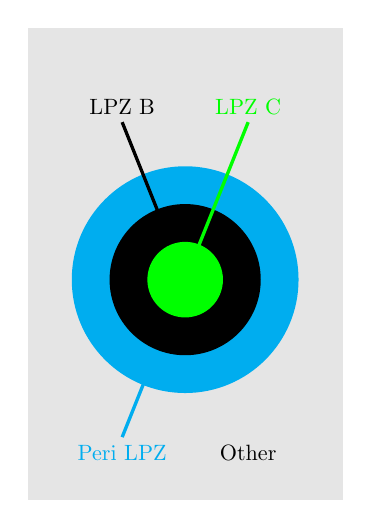
\begin{tikzpicture}[scale=0.8, transform shape]
  \fill [fill=black, thick, opacity=0.10] (0,0) rectangle ++(5,7.5);
  \node [below, black] at (3.5, 1.0){Other};

  \fill [cyan, opacity=1.0] (2.5, 3.5) circle (3.0*\radiuscircle);
  \draw [cyan, very thick] (1.5, 1.0)--(2.5, 3.5);
  \node [below, cyan] at (1.5, 1.0){Peri LPZ};

  \fill [black, opacity=1.0] (2.5, 3.5) circle (2.0*\radiuscircle);
  \draw [black, very thick] (1.5, 6.0)--(2.5, 3.5);
  \node [above, black] at (1.5, 6.0){LPZ B};

  \fill [green, opacity=1.0] (2.5, 3.5) circle (\radiuscircle);
  \draw [green, very thick] (3.5, 6.0)--(2.5, 3.5);
  \node [above, green] at (3.5, 6.0){LPZ C};

\end{tikzpicture}
